\documentclass[12pt,a4paper,dvipdfmx,fleqn]{article}%[a4paper,12pt,dvipdfmx,fleqn]{jarticle}
\setlength{\columnseprule}{0.4pt}
\setlength{\columnsep}{4zw} 
\setlength{\columnwidth}{5mm}
\usepackage[dvipdfmx]{graphicx,color}
\usepackage[top=25mm,bottom=25mm,left=20mm,right=20mm]{geometry}
\usepackage{amsmath,amsthm,amssymb,esvect,amsfonts,fancybox,tikz,tikz-3dplot,ulem,fancyhdr}
\usepackage{./sty/eclbkbox,./sty/okumacro,./sty/ascolorbox}
\usetikzlibrary{patterns,intersections,calc,quotes,angles,arrows.meta,positioning,graphs,through}
\tcbuselibrary{raster,skins,theorems,breakable}
\allowdisplaybreaks
\usepackage[dvipdfmx]{hyperref}
\usepackage{pxjahyper}
\hypersetup{% hyperrefオプションリスト
    setpagesize=false,
    bookmarksnumbered=true,%
    bookmarksopen=true,%
    colorlinks=true,%
    linkcolor=blue,
    citecolor=red,
}
\usepackage[absolute,overlay]{textpos}
\usepackage{ceo}
\usepackage{epic,eepic,emath,emathW,emathB,emathBk,emathMw,emathCap,emathE}
% =,→ 間の余白
\thickmuskip=1.0\thickmuskip
% +,- 間の余白
\medmuskip=0.8\medmuskip
% … などの装飾記号の余白
\thinmuskip=0.8\thinmuskip
% 行列を詰める
\arraycolsep=0.3\arraycolsep
% 数式の上下のスペースの変更
\AtBeginDocument{
    \abovedisplayskip     =0.5\abovedisplayskip
    \abovedisplayshortskip=0.5\abovedisplayshortskip
    \belowdisplayskip     =0.5\belowdisplayskip
    \belowdisplayshortskip=0.5\belowdisplayshortskip}
\usepackage{listings}
\lstset{
  basicstyle={\ttfamily},
  identifierstyle={\small},
  commentstyle={\smallitshape},
  keywordstyle={\small\bfseries},
  ndkeywordstyle={\small},
  stringstyle={\small\ttfamily},
  frame={tb},
  breaklines=true,
  columns=[l]{fullflexible},
  numbers=left,
  xrightmargin=0zw,
  xleftmargin=3zw,
  numberstyle={\scriptsize},
  stepnumber=1,
  numbersep=1zw,
  lineskip=-0.5ex
}
\pagestyle{fancy}
\lhead{競技プログラミングの鉄則 アルゴリズム力と思考力を高める77の技術}
\chead{}
\rhead{\thepage}
\cfoot{}
\theoremstyle{definition}
\newtheorem*{toi*}{問題}
\theoremstyle{definition}
\newtheorem*{ans*}{解説}
\theoremstyle{definition}
\newtheorem*{proof*}{証明}
\newcommand{\toukou}[2]{\begin{ascolorbox19}{第#1問}#2\end{ascolorbox19}}
\newcommand{\mybox}[1]{\,\raisebox{-.8ex}{\framebox(1.5em,1.5em)[c]{$#1$}}\,} %文字囲い
\newcommand{\ttt}[1]{\texttt{#1}} %文字囲い
\title{競技プログラミングの鉄則\thanks{\url{https://atcoder.jp/contests/tessoku-book}}}
\author{やさしい理系お兄ちゃん}
\date{\today}
\begin{document}
\begin{textblock*}{.5\textwidth}(5mm,20mm)
    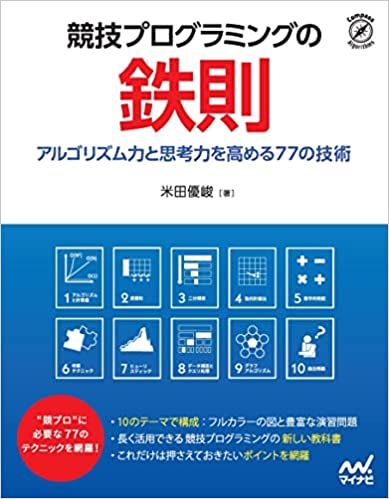
\includegraphics[width=4cm]{logo.jpg}
\end{textblock*}
\maketitle
\tableofcontents
\clearpage
\setcounter{section}{-1}
\section{はじめに}\label{はじめに}
このPDFは関数型言語Haskellの習得のために、「競技プログラミングの鉄則」の問題に対してHaskellで記述したコード例をまとめた資料です。
私のプログラミング力の向上を主目的とし、Haskellを学びたい人への手助けとなると良いと考えています。HaskellのI/O\footnote{I/O : Input(標準入力), Output(標準出力)}は一筋縄でいかないので、アルゴリズム
以前の問題で苦戦してしまうかもしれないでしょう。ですが、入出力に時間を取られるのは勿体無いため、そのような面でもHaskell習得の支えになれば良いと願います。
\section{アルゴリズムと計算量}\label{アルゴリズムと計算量}
\subsection{導入問題}\label{導入問題}
\begin{toi*}
    整数$N$が与えられるので、一辺の長さが$N$であるような正方形の面積を出力するプログラムを作成してください。
\end{toi*}
\begin{lstlisting}[caption=A01.hs,label=A01]
main :: IO ()
main = do
    n <- readLn :: IO Int
    putStrLn $ show (n * n)
\end{lstlisting}
\begin{ans*}
    \ttt{readLn}の型は\ttt{Read a => IO a}です。ここで、\ttt{:: IO Int}と後ろに記述することで型変数\ttt{a}は\ttt{Int}型であると宣言することができます。
    もちろん、書かなくても\ttt{(*)}という演算が後ろで行われていることから、型クラス\ttt{Num}に属することを推論してくれます。
    (書いた方が見やすいのではないでしょうか?)\ttt{n <- readLn :: IO Int}を実行すると、\ttt{n}は通常の整数値になります。
    \ttt{show}の型は\ttt{Show a => a -> String}であるから、\ttt{n * n}の結果を\ttt{show}に渡すことで、整数値を文字列に変換することができます。
    最後に\ttt{String -> IO ()}という型をもつ\ttt{putStrLn}に渡せば完了です。
\end{ans*}
\begin{toi*}
    整数$A$と$B$が与えられるので、$A+B$の値を出力するプログラムを作成してください。ただし、制約は$1\ll A\ll 100$、$1\ll B\ll 100$であるとします。
\end{toi*}
\begin{lstlisting}[caption=B01.hs,label=B01]
main :: IO ()
main = do
    [a, b] <- map read . words <$> getLine
    putStrLn $ show (a + b)
\end{lstlisting}
\begin{ans*}
    まずは2つの空白区切りの整数の入力から説明します。\ttt{<\$>}について、定義は以下の通りです。
    \begin{verbatim}
    (<$>) :: (Functor f) => (a -> b) -> f a -> f b
    f <$> x = fmap f x
    \end{verbatim}
    \vspace*{-4mm}
    \ttt{<\$>}の型に注目して下さい。\ttt{IO}は\ttt{Functor}のインスタンスであるから、\ttt{f}を\ttt{IO}に置き換えると、
    \ttt{<\$> :: (a -> b) -> IO a -> IO b}となります。
    また、
    \begin{itemize}
        \item [] \ttt{getLine :: IO String}
        \item [] \ttt{map read . words :: Read b => String -> [b]}
    \end{itemize}
    と定義されています。以上を合わせると
    \begin{verbatim}
    map read . words <$> getLine :: (Read b) => IO [b]
    \end{verbatim}
    \vspace*{-4mm}
    となることが分かります。\ttt{IO [b]}については、コンパイラが勝手に\ttt{IO [Int]}としてくれます。\footnote{Type Defaultingというものが使われています。詳しくはいつか書きます。(\today)}
    当然、\ttt{:: IO {Int}}と型を指定するのもいいことでしょう。最終的に、結果を\ttt{Int}型のリストとして\ttt{[a, b]}に束縛することができます。(\chub 入力が2つであると分かっているので、\ttt{[a, b]}としています。)
    あとは計算結果をA01と同様に出力すれば完了です。
\end{ans*}
\subsection{全探索1}\label{全探索1}
\begin{toi*}
    $N$個の整数$A_1,\,A_2,\,\udots,\,A_N$の中に、整数$X$が含まれるかどうかを判定するプログラムを作成してください。
\end{toi*}
\begin{lstlisting}[caption=A02.hs,label=A02]
main :: IO ()
main = do
    [n, x] <- map read . words <$> getLine :: IO [Int]
    as <- map read . words <$> getLine :: IO [Int]
    putStrLn $ if x `elem` as then "Yes" else "No"
\end{lstlisting}
\begin{ans*}
    3, 4行目に関してはListing~\ref{B01}の解説で紹介しました。そろそろ気付いたかもしれませんが、Haskellでは\texttt{for}を使った繰り返し処理を
    行わないので、リストの長さを示す\texttt{n}を受け取る必要がないことが多いです。そのため、3行目は
    \begin{verbatim}
    [_, x] <- map read . words <$> getLine
    \end{verbatim}
    \vspace*{-4mm}
    としても良いです。そして、リスト\texttt{as}の中に\texttt{x}が含まれているかは、関数\texttt{elem}で判定することができます。
    関数\texttt{elem}は中置記法を用いることが多いです。
\end{ans*}
\begin{toi*}
    $A$以上$B$以下の整数のうち、100の約数であるものは存在しますか。答えをYesかNoで出力するプログラムを作成してください。
\end{toi*}
\begin{lstlisting}[caption=B02.hs,label=B02]
main :: IO ()
main = do
    [a, b] <- map read . words <$> getLine :: IO [Int]
    let x = [a..b]
    putStrLn $ if 0 `elem` map (100 `mod`) x then "Yes" else "No"
\end{lstlisting}
\begin{ans*}
    4行目の\texttt{[a..b]}は、\texttt{[a, a+1, a+2, ..., b-1, b]}を表します。
    このリストのすべての要素について、100から割った余りを考えます。その余りのリストの中に\texttt{0}が含まれてるか否かを判定します。
\end{ans*}
\subsection{全探索2}\label{全探索2}
\begin{toi*}
    赤いカードが$N$枚あり、それぞれ整数$P_1,\,P_2,\,\udots,\,P_N$が書かれています。また、青いカードが$N$枚あり、それぞれ整数$Q_1,\,Q_2,\,\udots,\,Q_N$が書かれています。
    太郎くんは、赤いカードの中から1枚、青いカードの中から1枚、合計2枚のカードを選びます。選んだ2枚のカードに書かれた整数の合計が$K$となるようにする方法は存在しますか。答えを出力するプログラムを書いてください。
\end{toi*}
\begin{lstlisting}[caption=A03.hs,label=A03]
main :: IO ()
main = do
    [_, k] <- map read . words <$> getLine :: IO [Int]
    ps <- map read . words <$> getLine :: IO [Int]
    qs <- map read . words <$> getLine :: IO [Int]
    putStrLn $ if k `elem` [p + q | p <- ps, q <- qs] then "Yes" else "No"
\end{lstlisting}
\begin{ans*}
    6行目の
    \begin{verbatim}
    [p + q | p <- ps, q <- qs]
    \end{verbatim}
    \vspace*{-4mm}
    では、リスト\texttt{ps}とリスト\texttt{qs}から一つずつ要素を取り出し、それらを足し合わせて可能性のある答えをすべて計算して提示しています。
    これを{\bf 非決定性計算}とみなすことができます。このとき、
    \begin{verbatim}
    (+) <$> ps <*> qs
    \end{verbatim}
    \vspace*{-4mm}
    と書くことができます。これについては{\bf アプリカティブ}という用語を聞くまでは保留で構いません。非決定性計算という言葉も同様です。
    (いずれ、後者の記法の方がきれいだと感じる日が来るはずです!私はまだ来ていませんが。)
\end{ans*}
\begin{toi*}
    $N$個の商品があり、商品$i~(1\ll i\ll N)$の価格は$A_i$円です。異なる3つの商品を選び、合計価格をピッタリ1000円
    にする方法は存在しますか。答えをYesかNoで出力するプログラムを作成してください。ただし、制約は$3\ll N\ll 1000$であるとします。
\end{toi*}
\begin{lstlisting}[caption=B03.hs,label=B03]
just :: Int -> Int -> [Int] -> Bool
just _ _ [] = False
just 1 num xs = num `elem` xs
just 2 num (x : xs) = any (\m -> m + x == num) xs || just 2 num xs
just k num as@(x : xs) = length as >= k && k >= 0
    && (just (k - 1) (num - x) xs || just k num xs)

main :: IO ()
main = do
    _ <- read <$> getLine :: IO Int
    as <- map read . words <$> getLine :: IO [Int]
    putStrLn $ if just 3 1000 as then "Yes" else "No"
\end{lstlisting}
\begin{ans*}
    本問も非決定性計算だから、Listing~\ref{A03}と同様に
    \begin{verbatim}
    1000 `elem` [x + y + z | x <- as, y <- as, z <- as]
    \end{verbatim}
    \vspace*{-4mm}
    で可能性のある答えを列挙しよう!としては...方針は正しいですが、その手法に誤りが生じています。
    これでは、同じ商品を選ぶ場合も含まれてしまうからです。\par
    それでは、関数\texttt{just}について説明します。
    \texttt{just k num xs}とは、リスト\texttt{xs}から、異なる\texttt{k}個の要素を取り出して足し合わせたとき、
    その答えが\texttt{num}になることがあるか否かを示す式です。したがって、本文では入力から得たリストに\texttt{just 3 1000}を適用します。
    \begin{enumerate}
        \item [$\maruichi$] \texttt{just \_ \_ []}\\
            リストが空なら、問答無用で\texttt{False}を返します。
        \item [$\maruni$] \texttt{just 1 num xs}\\
            リストから1個だけ取り出して、\texttt{num}に等しいかを判定します。おなじみの関数\texttt{elem}を使えば解決です。
        \item [$\marusan$] \texttt{just 2 num xs}\\
            まず、\texttt{any (\symbol{`\\}m -> m + x == num) xs}で、先頭要素とその他の要素を足して\texttt{num}になるかを判定しています。
            そこで、\texttt{True}が得られなかった場合、\texttt{just 2 num xs}で先頭要素を捨てて残りのリストで同じことを試します。
            以降、再帰的に判定します。
        \item [$\marushi$] \texttt{just k num xs}\\
            \texttt{k}個取り出すので、\texttt{k}が負でないこと、リストの長さが\texttt{k}以上であることを判定しておきます。(\chub このような判定を書かずとも、
            AtCoderでは正しい入力が与えられることが保証されているので問題ありません。しかし、一般的にはそうではないので、意図せぬ入力にも備えておく癖をつけましょう!
            とは言っても、AtCoderではこれを書くのは手間ですので、やっぱり以降はサボります。)\par
            あとは、$\marusan$と同様に、まずは先頭要素とその他の要素について条件を満たす組合せが存在するかを判定します。このとき、
            \texttt{just (k - 1) (num - x) xs}に帰着されることを理解しましょう。
    \end{enumerate}
\end{ans*}
\subsection{2進法}\label{2進法}
\begin{toi*}
    整数$N$が10進法表記で与えられます。$N$を2進法に変換した値を出力するプログラムを作成してください。
\end{toi*}
\begin{lstlisting}[caption=A04.hs,label=A04]
toBinary :: Int -> String
toBinary 1 = "1"
toBinary n = toBinary (n `div` 2) ++ if even n then "0" else "1"

assignZero :: Int -> String -> String
assignZero 0 str = str
assignZero x str = "0" ++ assignZero (x - 1) str

main :: IO ()
main = do
    n <- readLn :: IO Int
    let binary = toBinary n
    putStrLn $ assignZero (10 - length binary) binary
\end{lstlisting}
\begin{ans*}
    関数\texttt{toBinary}の動きを見てみましょう。
    \begin{verbatim}
    toBinary 12 -> toBinary 6 ++ "0" -> toBinary 3 ++ "00"
                -> toBinary 1 ++ "100" -> "1100"
    \end{verbatim}
    \vspace*{-4mm}
    どうでしょう?2進数を計算する方法は数Aで習いますね!
\end{ans*}
\begin{toi*}
    整数$N$~(8桁以内)が2進法表記で与えられます。$N$を10進法に変換した値を出力するプログラムを作成してください。
\end{toi*}
\begin{lstlisting}[caption=B04.hs,label=B04]
bin2list :: Int -> [Int] -> [Int]
bin2list 0 ys = ys
bin2list x ys = bin2list (x `div` 10) (x `mod` 10 : ys)

list2dec :: [Int] -> Int
list2dec [] = 0
list2dec (x : xs) = x * (2 ^ length xs) + list2dec xs

main :: IO ()
main = do
    n <- readLn :: IO Int
    print $ list2dec $ bin2list n []
\end{lstlisting}
\begin{ans*}
    与えられた入力(例えば101011)を
    \begin{verbatim}
    101011 -> [1,0,1,0,1,1] -> 2^5 + 2^3 + 2^1 + 2^0 -> 43
    \end{verbatim}
    \vspace*{-4mm}
    という流れで計算しています。入力を\texttt{Int}として受け取り、それをリスト構造に変換しているなら、
    最初からリスト構造である\texttt{String}で受け取るべきですね。\par
    おっと、関数\texttt{print}が初登場しました。型は以下のようになっています。
    \texttt{putStrLn}との違いを見てみましょう。
    \begin{verbatim}
    print :: Show a => a -> IO ()
    putStrLn :: String -> IO ()
    \end{verbatim}
    \vspace*{-4mm}
\end{ans*}
\subsection{チャレンジ問題}\label{チャレンジ問題1}
\begin{toi*}
    赤・青・白の3枚のカードがあります。太郎くんは、それぞれのカードに1以上$N$以下の整数を書かなければなりません。
    3枚のカードの合計を$K$にするような書き方は何通りありますか。
\end{toi*}
\begin{lstlisting}[caption=A05.hs,label=A05]
main :: IO ()
main = do
    [n, k] <- map read . words <$> getLine :: IO [Int]
    print $ length [(a, b, c) | a <- [1..n], b <- [1..n], let c = k - a - b, 1 <= c, c <= n]
\end{lstlisting}
\begin{ans*}
    リスト内包表記のおかげで解説いらず!\texttt{1}以上\texttt{n}以下の範囲で、\texttt{a + b + c = k}となるように\texttt{c}を定めてあげます。
    出来上がったトリプルのリストの長さが答えになります。
\end{ans*}
\section{累積和}\label{累積和}
\subsection{一次元の累積和}\label{一次元の累積和}
\begin{toi*}
    ある遊園地では$N$日間にわたるイベントが開催され、$i$日目には$A_i$人が来場しました。
    以下の$Q$個の質問に答えるプログラムを作成してください。
    \begin{itemize}
        \item [] 質問1:$L_1$日目から$R_1$までの来場者数は?\\[2mm]
        \hspace{2em}{\vdots}
        \item [] 質問$Q$:$L_Q$日目から$R_Q$までの来場者数は?
    \end{itemize}
\end{toi*}
\begin{lstlisting}[caption=A06\_00.hs,label=A06_00]
import Control.Monad ( replicateM_ )

cumulativeSum :: [Int] -> [Int]
cumulativeSum = scanl (+) 0

solve :: [Int] -> [Int] -> Int
solve s [l, r] = (s !! r) - (s !! (l - 1))

main :: IO ()
main = do
    [_, q] <- map read . words <$> getLine :: IO [Int]
    as <- map read . words <$> getLine :: IO [Int]
    let cumSum = cumulativeSum as
    replicateM_ q $ do
        lr <- map read . words <$> getLine :: IO [Int]
        print $ solve cumSum lr
\end{lstlisting}
\begin{ans*}
    新しい関数がたくさん登場しました。一つずつ紹介します。\par
    関数\texttt{scanl}の定義は以下です。
    \begin{verbatim}
    scanl :: (b -> a -> b) -> b -> [a] -> [b]
    scanl = scanlGo
        where
            scanlGo :: (b -> a -> b) -> b -> [a] -> [b]
            scanlGo f q ls = q : (case ls of
                            []   -> []
                            x:xs -> scanlGo f (f q x) xs)
    \end{verbatim}
    \vspace*{-4mm}
    なぜ、\texttt{scanlGo}を挟んでいるのか!?(2023年12月16日:実力不足によりまだわかっておりません。)
    実装自体は理解できそうですね!動作を見てみましょう。
    \begin{verbatim}
    scanl (+) 0 [1,2,3,4,5] -> [0,1,3,6,10,15]
    \end{verbatim}
    \vspace*{-4mm}
    これがまさに累積和になります。引数のリストの長さを$N$とすると、関数\texttt{cumulativeSum}は$O(N)$となります。
    上記の例で考えると、2日目から4日目までの来場者数は、\texttt{10 - 1 = 9}(人)となります。3日目から5日目までの来場者数は、
    \texttt{15 - 3 = 12}(人)となります。\par
    リストの\texttt{k}番目の要素にアクセスするために関数\texttt{(!!)}が使えます。したがって、質問に回答する関数\texttt{solve}
    は
    \begin{verbatim}
    solve s [l, r] = (s !! r) - (s !! (l - 1))
    \end{verbatim}
    \vspace*{-4mm}
    と定義できます。(「0日目は累計0人」という無意味な情報をリストの先頭に置いておくことで、リストのインデックスと日にちの数字が同じ数字になるので扱いやすくなっています。)
    これを、関数\texttt{replicateM\_}を用いて\texttt{q}個の質問に適用します。ここでは、使用例だけ紹介します。
    \begin{verbatim}
    ghci> replicateM_ 3 (putStrLn "a")
    a
    a
    a
    \end{verbatim}
    \vspace*{-4mm}
    \par
    これで完成!いえ、実行時間超過です。なぜでしょう... オーダーに問題があります。プログラムとしては正しい出力が得られます。
    このプログラムは$O(N^2)$であり、$0\ll N\ll 10^5$から、最悪計算量が$10^{10}$となってしまうため制限時間超過となります。問題文では、
    $O(N+Q)$であることが望ましいと書かれていますので、それを目標にプログラムを変更しましょう。\par
    関数\texttt{cumulativeSum}は$O(N)$で、関数\texttt{replicateM\_}は$O(Q)$です。したがって、関数\texttt{(!!)}が$O(1)$であれば、非常に嬉しい!ということになります。
    しかしながら、$O(N)$であるようです。下記の定義からも確認できますね。
    \begin{verbatim}
    (!!) :: [a] -> Int -> a
    xs     !! n | n < 0 =  errorWithoutStackTrace 
                                "Prelude.!!: negative index"
    []     !! _         =  errorWithoutStackTrace 
                                "Prelude.!!: index too large"
    (x:_)  !! 0         =  x
    (_:xs) !! n         =  xs !! (n-1)
    \end{verbatim}
    \vspace*{-4mm}
    では、$O(1)$で配列の要素にアクセスするにはどうしたらよいのでしょうか? \texttt{Data.Array}モジュールを使いましょう。
\end{ans*}
\begin{lstlisting}[caption=A06\_01.hs,label=A06_01]
import Control.Monad ( replicateM_ )
import Data.Array ( Array, (!), elems, listArray )

cumulativeSum :: Int -> Int -> Array Int Int -> Array Int Int
cumulativeSum l r as = listArray (l, r) $ scanl (+) 0 $ elems as

solve :: Array Int Int -> [Int] -> Int
solve s [l, r] = (s ! r) - (s ! (l - 1))

main :: IO ()
main = do
    [n, q] <- map read . words <$> getLine :: IO [Int]
    as <- listArray (0, n - 1) . map read . words <$> getLine :: IO (Array Int Int)
    let cumSum = cumulativeSum 0 n as
    replicateM_ q $ do
        lr <- map read . words <$> getLine :: IO [Int]
        print $ solve cumSum lr
\end{lstlisting}

% \begin{toi*}
%     太郎君はくじを$N$回引き、$i$回目の結果は$A_i$でした。$A_i=1$のときアタリ、$A_i=0$のときハズレを意味します。
%     「$L$回目から$R$回目までの中では、アタリとハズレどちらが多いか?」という形式の質問が$Q$個与えられるので、
%     それぞれの質問に答えるプログラムを作成してください。計算量は$O(N+Q)$であることが望ましいです。
% \end{toi*}
% \begin{lstlisting}[caption=B06.hs,label=B06]
% \end{lstlisting}
% \begin{ans*}
% \end{ans*}
% \begin{toi*}
%     ある会社ではD日間にわたってイベントが開催され、N人が出席します。参加者$i$は$L_i$日目から$R_i$日目まで出席する予定です。
%     各日の出席者数を出力するプログラムを作ってください。
% \end{toi*}
\end{document}